\documentclass[12pt]{article}

\usepackage{chngcntr}
\counterwithin{figure}{section}
\counterwithin{table}{section}

\usepackage{qtree}
\usepackage{tikz}
\usepackage{tikz-qtree}
\usepackage{textcomp}
\usetikzlibrary{positioning, shapes.geometric}

\usepackage[utf8]{inputenc}
\usepackage[T1]{fontenc}
\usepackage[french]{babel}
\usepackage[a4paper, margin=2cm]{geometry}
\usepackage{wrapfig}
\usepackage{titlesec}

\setcounter{secnumdepth}{4}

\usepackage{cite}

\usepackage{listings}
\usepackage{color}
\definecolor{dkgreen}{rgb}{0,0.6,0}
\definecolor{gray}{rgb}{0.5,0.5,0.5}
\definecolor{mauve}{rgb}{0.58,0,0.82}
\definecolor{Darkblue}{rgb}{0,0,0.5}

\usepackage{algorithm}
\usepackage{algorithmicx}
\usepackage{algpseudocode}
\usepackage{amsmath,amssymb,amsfonts}
\floatname{algorithm}{Algorithm} 
\renewcommand{\algorithmicrequire}{\textbf{Input:}} 
\renewcommand{\algorithmicensure}{\textbf{Output:}} 

\usepackage{hyperref}
\hypersetup{
    colorlinks=true,
    linkcolor=Darkblue,
    filecolor=magenta,      
    urlcolor=cyan,
    pdfpagemode=FullScreen,
    }

\lstset{frame=tb,
  language=C,
  aboveskip=3mm,
  belowskip=3mm,
  showstringspaces=false,
  columns=flexible,
  basicstyle={\small\ttfamily},
  numbers=none,
  numberstyle=\tiny\color{blue},
  keywordstyle=\color{blue},
  commentstyle=\color{blue},
  stringstyle=\color{mauve},
  breaklines=true,
  breakatwhitespace=true,
  tabsize=3,
  numbers=left,
  numbersep=10pt
}


\usepackage{fancyhdr}
\pagestyle{fancy}
\renewcommand{\headrulewidth}{0pt}
\fancyhead[C]{} 
\fancyhead[L]{}
\fancyhead[R]{}

\renewcommand{\footrulewidth}{1pt}
\fancyfoot[C]{Simulation - TP 4\\\textbf{Page \thepage/\pageref{lastPage}}}
\fancyfoot[L]{Ao XIE \\ Chloé BERTHOLD}
\fancyfoot[R]{ISIMA}


\usepackage{array,multirow,makecell}
\setcellgapes{1pt}
\makegapedcells
\newcolumntype{R}[1]{>{\raggedleft\arraybackslash }b{#1}}
\newcolumntype{L}[1]{>{\raggedright\arraybackslash }b{#1}}
\newcolumntype{C}[1]{>{\centering\arraybackslash }b{#1}}

\begin{document}
    \def\arraystretch{1.5}
        
\includegraphics[scale = 0.8]{Photos/isima.jpg}  
        \hfill
        \begin{large}
            Enseignant : David HILL
        \end{large}
        
    \vspace{3cm}
    \begin{center}
        \begin{Huge}
            \textbf{Simulation ZZ2 - TP 4}
            \\
            \vspace{0.3cm}
            \textbf{Rabbit Population Growth}
        \end{Huge}
    \end{center}
    
    \begin{center}
        \begin{large}
            Ao XIE \& Chloé BERTHOLD - Décembre 2022
        \end{large}
    \end{center}
    
    \vspace{1.5cm}
	\begin{center}
	    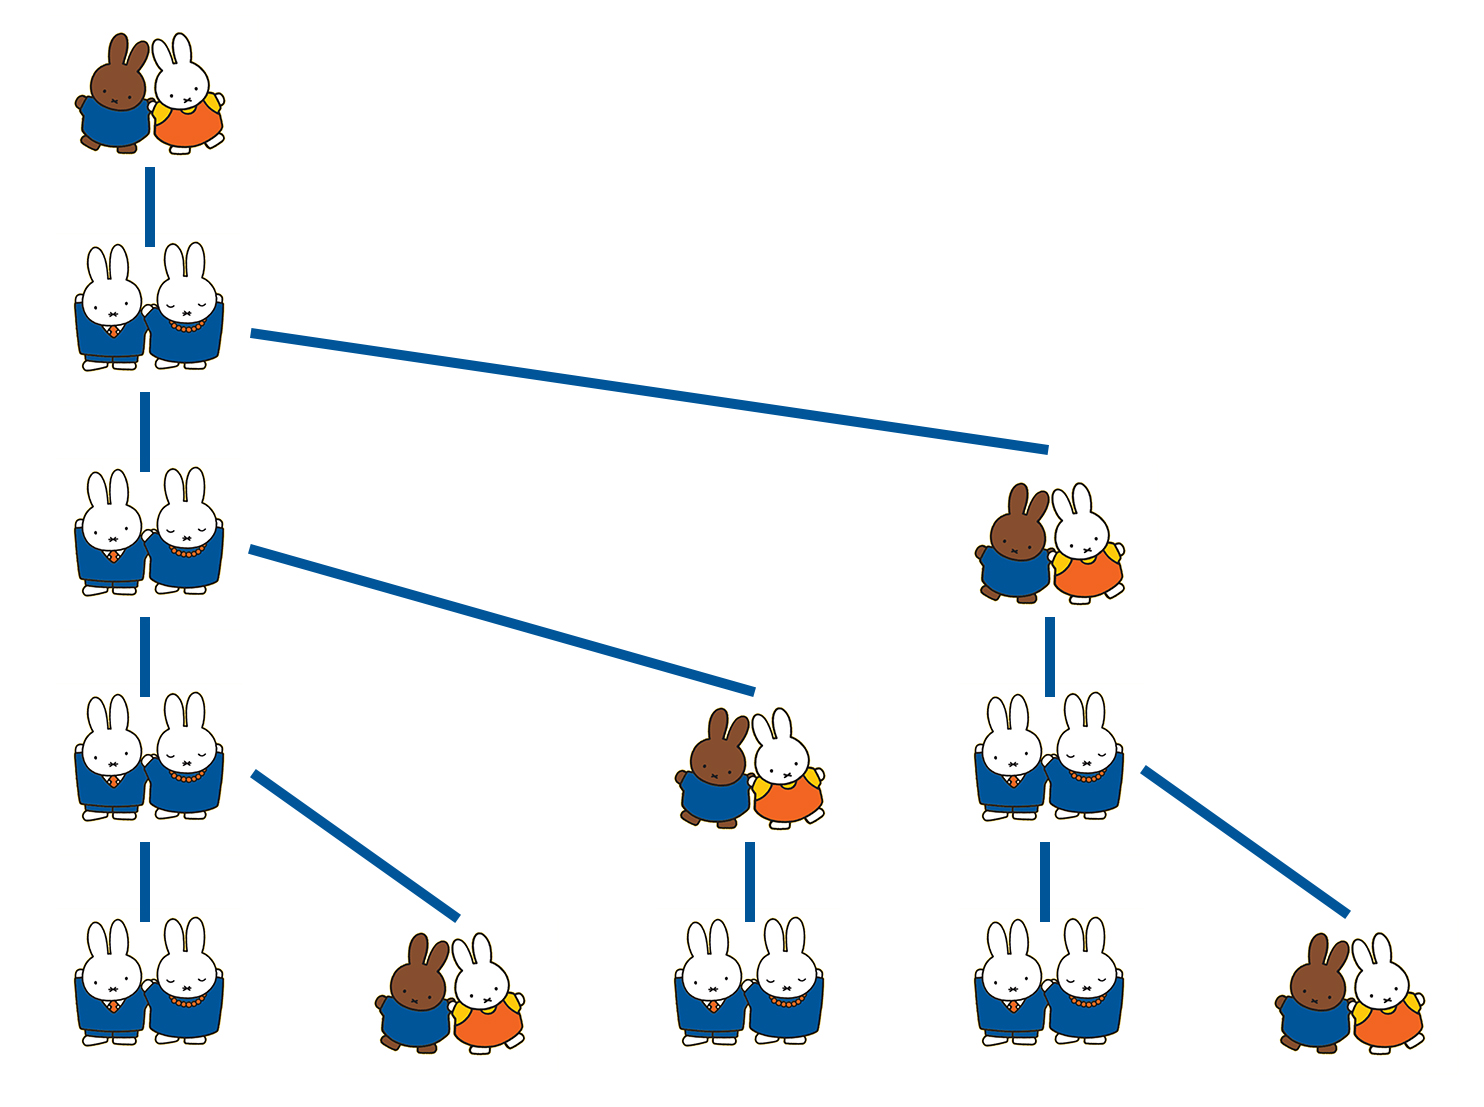
\includegraphics[width=15cm]{Photos/Miffy_Fibonacci.jpg}
	\end{center}

    \vspace{1cm}
    \begin{center}
        \begin{small}
            Campus des Cézeaux, 1 rue de la Chébarde, TSA 60125, 63178 Aubière CEDEX
        \end{small}
    \end{center}
    \thispagestyle{empty}
%1er page fini%    
    \newpage
    \begin{center}
    \section*{Introduction}    
    \end{center}
    \par
    Leonardo Fibonacci, dans le livre de calcul\cite{Sigler:2002:FLA}, a posé un problème de croissance des lapins dans des conditions idéales. Dans ce problème, les lapins suivent une des règles de veillissement itératives, c'est-à-dire qu'une paire de lapins juvéniles évolue en une paire de lapins adultes après une itération, et une paire de lapins adultes donne naissance à une paire de lapins juvéniles après une itération. Dans cette hypothèse, le nombre de lapins évolu ainsi : 2, 3, 5, 8, 13, 21, 34, 55, 89... Cette série est donc connue sous le nom de série de Fibonacci. Elle est caractérisée par le fait que chaque valeur de la séquence est égale à la somme des deux valeurs précédentes.
    \par La séquence de Fibonacci a des applications qui vont bien au-delà du calcul du nombre de lapins dans un environnement idéal ; il existe également un grand nombre de séquences de Fibonacci dans la nature\cite{minarova2014fibonacci}. En 2002, AJS Klar et al. ont suggéré que le nombre d'hélices dans le triage en spirale des tiges et des feuilles, des pétales et des têtes de fleurs au cours du développement des plantes est conforme à la séquence de Fibonacci\cite{klar2002plant}. Dans le domaine des applications, l'impact de la série de Fibonacci a été beaucoup plus important. En 2004, E Karaduman et al. ont appliqué la série de Fibonacci au déterminant matriciel de la série de Fibonacci d'ordre k généralisé\cite{karaduman2004application}. La même année, J Zou et RK Ward et al. ont appliqué les transformées de Fibonacci généralisées à des permutations d'images et ont constaté que celles-ci présentaient des propriétés d'uniformité souhaitables\cite{zou2004generalized}. Et en 2017, S Sinha et al. ont appliqué la série de Fibonacci au domaine du chiffrement après avoir résumé ses caractéristiques pour améliorer la sécurité du chiffrement\cite{sinha2017fibonacci}.
    \par Dans cet article, nous revenons sur les origines de la séquence de Fibonacci, par opposition à son application dans d'autres domaines. Nous mettons d'abord en œuvre une simulation de la population de lapins dans des conditions idéales en utilisant le langage C, une situation qui recrée l'idée originale de Fibonacci. Immédiatement après, nous avons modifié ce cadre idéal pour le rapprocher de la réalité. Ainsi, nous avons réalisé une simulation de la population de lapins qui est proche des conditions réalistes.
%2eme page fini%
    \newpage
	\tableofcontents
    
    \newpage
    \listoftables
    \listoffigures
%3eme page fini%
    \newpage
    \section{Présentation générale}
    Dans cette section, nous présentons les règles pour la simulation de la taille de cette population de lapins, puis les idées pour notre approche finale de mise en œuvre.
        \subsection{Rappel des objectifs}
        Après avoir réalisé un algorithme de Fibonacci simple, les hypothèses suivantes sont faites afin de rendre le nombre de lapins de la colonie plus réaliste : 
        \begin{itemize}
            \item 1. Chaque lapine donnera naissance à 3 à 6 ronds par an de manière uniformément répartie. Le nombre de lapins à chaque tour sera compris entre 4 et 8, ce qui est normalement distribué.
            \item 2. Les chances qu'un lapin nouveau-né soit une femelle ou un mâle sont de 50\% chacune.
            \item 3. Les jeunes lapins atteignent l'âge adulte entre cinq et huit mois, ou un an lorsque l'année est utilisée comme unité de calcul.
            \item 4. Les taux de survie sont de 35\% pour les lapins immatures et de 65\% pour les adultes, tandis qu'après l'âge de dix ans, le taux de survie diminue de 10\% chaque année.
        \end{itemize}
        
        \subsection{Méthode de réalisation}
        Pour mettre en œuvre cette simulation de la taille de la population de lapins, nous avons d'abord essayé d'utiliser le mois comme unité de calcul. Finalement, nous avons choisi d'utiliser l'année comme unité de calcul. C'est pourquoi, dans cette section, nous allons présenter les avantages et les inconvénients de ces deux unités et les raisons du choix final.
            \subsubsection{Mois comme unité de calcul}
            Initialement, afin d'améliorer la précision du processus de simulation de la population et d'obtenir un simulateur présentant des conditions d'ajustement maximales, nous avons utilisé le mois comme unité pour la simulation de la population de lapins. Cependant, les inconvénients de cette méthode de calcul sont vite apparus.
            \par
            Dans le processus d'utilisation de ce type de calcul, nous utilisons une structure comme objet, suivant les idées des langages orientés objet. Dans ce cas, nous pouvons atteindre un simulateur de très haute précision. Ensuite, un tableau de structures est utilisé pour stocker chaque propriété de chaque lapin. Et comme chaque lapin individuel nécessite une allocation distincte d'espace de stockage, même si l'espace occupé par le lapin mort est libéré à l'aide de la mémoire dynamique, après quarante à cinquante itérations, c'est-à-dire environ trois à quatre ans, il remplira la mémoire de l'ordinateur{\textcolor{blue}{*}} qu'il utilise et ne sera plus simulé. De plus, en raison du faible taux de survie des lapins à un jeune âge (35\%), un nombre énorme de lapins est nécessaire pour initialiser le simulateur, ce qui est proche de la limite de mémoire de l'ordinateur.
            \par
            Tant au niveau matériel qu'au niveau logiciel, avec cette limitation, nous avons finalement choisi d'utiliser l'année comme unité de calcul.
            \subsubsection{Année comme unité de calcul}
            Lorsque nous utilisons l'année comme unité de calcul pour le simulateur, notre approche consiste à ne plus utiliser les lapins comme objets et à utiliser des tableaux à la place. Nous utilisons l'index du tableau comme âge et les éléments du tableau pour indiquer le nombre de lapins de cet âge. Au total, nous utilisons deux tableaux, l'un pour stocker les lapins mâles et l'autre pour stocker les lapins femelles.
            \par
            Lorsque nous faisons cela, nous n'avons plus besoin de tenir compte des contraintes matérielles relatives à l'allocation et à l'utilisation de la mémoire, ni d'optimiser l'algorithme pour obtenir un peu plus de 50 itérations, mais uniquement du type des éléments du tableau, car c'est ce type d'élément qui, en fin de compte, affectera le nombre de lapins.
            \par
            Ainsi, lorsque nous utilisons l'année comme unité de calcul, le tableau que nous utilisons pour stocker le nombre de lapins est illustré dans la figure \ref{fig:rabbit}
            \begin{figure}[htbp]
                \centering
                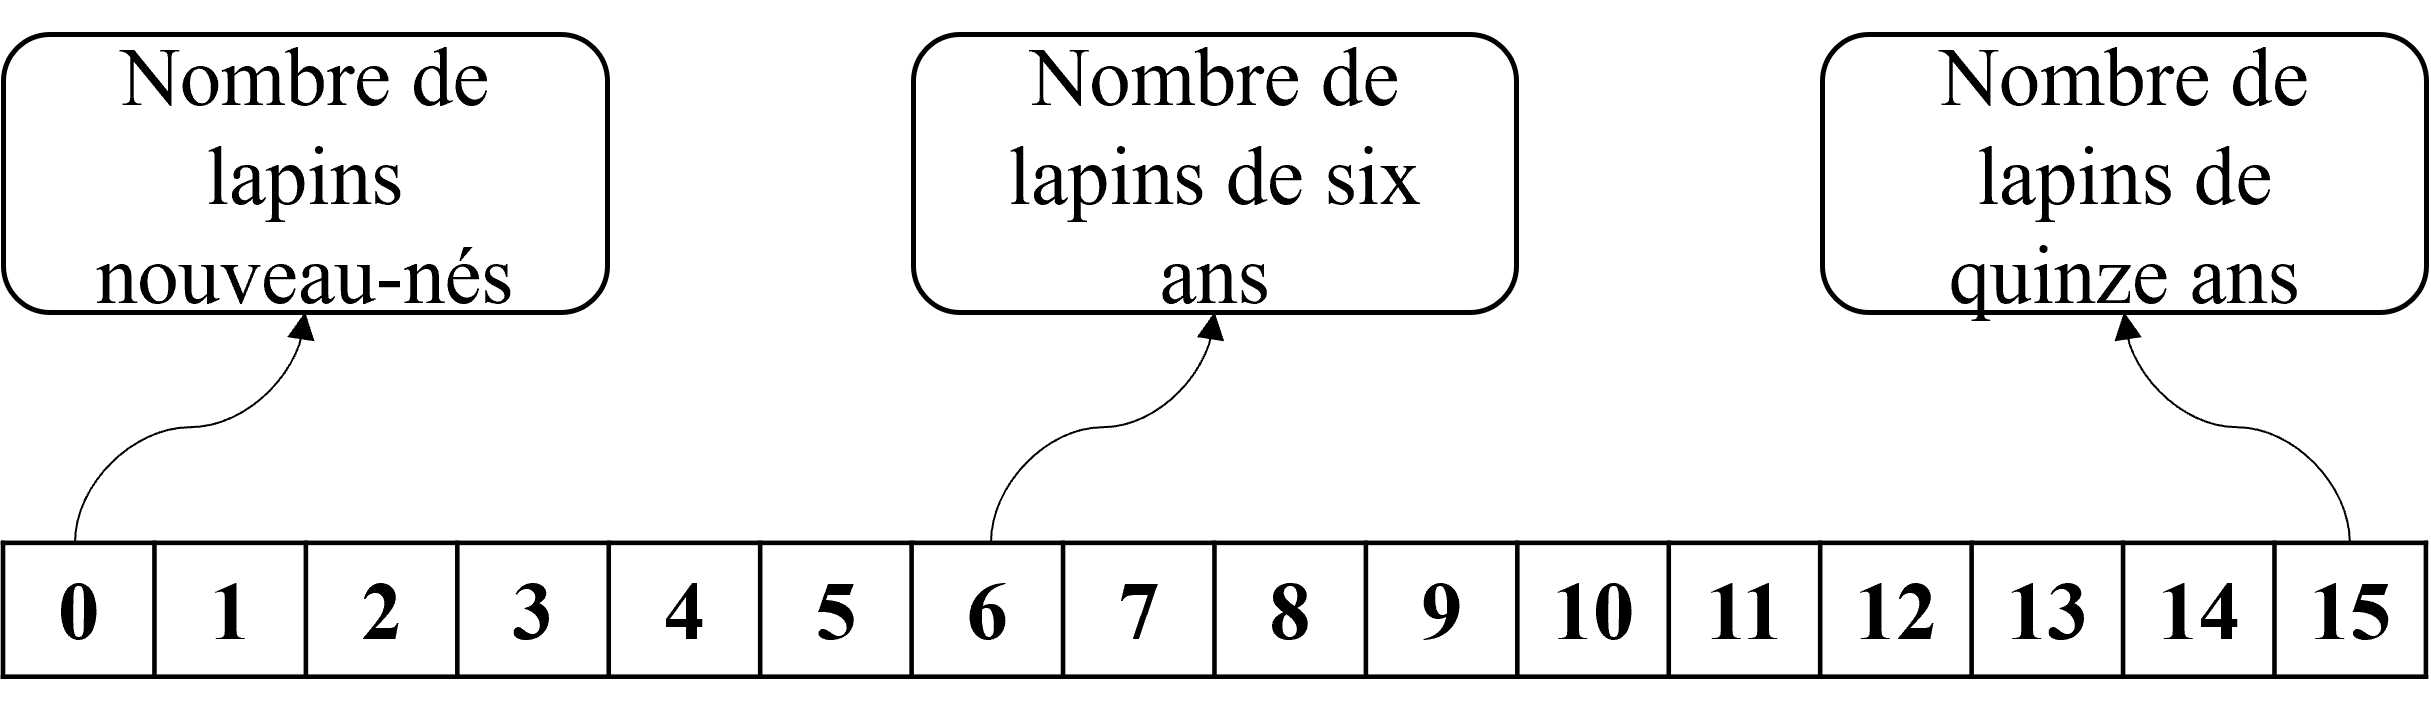
\includegraphics[scale=0.75]{Photos/Rabbit.png}
                \caption{Format de tableau pour le stockage des lapins}
                \label{fig:rabbit}
            \end{figure}

            \subsection{Organisation du code source}
	Ce TP est divisé en cinq fichiers :
	\begin{itemize}
	    \item Le fichier \emph{mt.h} qui regroupe les signatures de toutes les fonctions codées par Makoto Matsumoto.
	    \item Le fichier \emph{mt.c} où sont implémentées les fonctions définies dans le fichier \emph{mt.h}.
	    \item Le fichier \emph{lapins.h} qui regroupe les signatures des fonctions codées dans le cadre du TP.
	    \item Le fichier \emph{lapins.c} où sont implémentées les fonctions définies dans le fichier \emph{lapins.h}.
	    \item Le fichier \emph{main.c} qui contient la fonction main du programme et où sont réalisées dix simulations sur vingts ans.
	\end{itemize}
            
    \newpage    
	\section{Fonctions de développement}
        Dans cette section, nous expliquons les composants nécessaires à une simulation complète de la population de lapins et nous    les analysons. Si l'on exclut les parties restantes, l'ensemble de l'algorithme se compose de dix fonctions, qui sont les suivantes: \emph{judgeGender()}, \emph{timeSexualMat()}, \emph{calculChanceSurvival()}, \emph{BoxMuller()}, \emph{getTimesChildYear()}, \emph{getNbBaby()}, \emph{getDeaths()}, \emph{getAdultFemales()}, \emph{getAdultMale()}, \emph{realRabbit()}, \emph{oneYearLater} et \emph{multipleExperiments}. 
        \par 
        Pour ces fonctions, nous les avons divisées en deux catégories en fonction des besoins qu'elles remplissent: calcul du nombre de jeunes lapins nés et supprimer les lapins morts.
    
        \subsection{Calcul du nombre de jeunes lapins nés}
        Il s'agit d'un simulateur qui recherche des résultats réalistes. Nous essayons donc de simuler autant que possible l'état réel de la population de lapins. Par conséquent, dans ce simulateur, nous considérons que toutes les lapines peuvent encore se reproduire tant qu'il y a encore un lapin mâle adulte. Dans cette condition, notre algorithme de modélisation du nombre de lapins nés par an est présenté à la figure \ref{algo:birth}.
        \begin{figure}[htbp]
            \centering
            \label{algo:birth}
            \begin{algorithm}[H]
                \begin{algorithmic}[1]
                    \caption{Nombre de jeunes lapins nés}
                    \State $numAduletFemales \leftarrow getAdultFemales()$
                    \If{$stateMale >= 1$}
                        \For{$i = 1 \to numAduletFemales$}
                            \State $timeThisYear \leftarrow getTimeChildYear()$
                            \For{$j=0\to timeThisYear$}
                                \State $babyThisYear += getNbBaby() $
                            \EndFor
                        \EndFor
                        \For{$i=0 \to babyThisYear$}
                            \State $judgeGender()$
                            \State $babies[sex]++$
                        \EndFor
                    \EndIf
                \end{algorithmic}
            \end{algorithm}
            \caption{Algorithme pour le nombre de lapins de naissance} 
        \end{figure}
        
        \subsection{Supprimer les lapins morts}
        Dans cette section, nous itérons sur l'âge des lapins et utilisons l'âge des lapins pour calculer le taux de mortalité des lapins et ensuite mettre à jour le nombre de lapins. Ce que nous avons fait ici est d'ajuster le tableau dans lequel les lapins mâles et femelles sont situés en déplaçant les éléments du tableau d'une place en arrière, en supprimant le dernier élément original et en mettant le premier élément, le nombre de lapins nouvellement nés, à zéro. Cette partie consiste en une seule fonction, elle est  $getDeath()$, et son algorithme est présenté dans la figure \ref{algo:die}
        
        \begin{figure}[htbp]
            \centering
            \label{algo:die}
            \begin{algorithm}[H]
                \begin{algorithmic}[1]
                    \Require start
                    \caption{getDeath()}
                    \State $start \Rightarrow females[15] \leftarrow 0$
                    \State $start \Rightarrow males[15] \leftarrow 0$
                    \For{$age=14\to -1$}
                        \For{$rabbit=0 \to start\Rightarrow females[age]$}
                            \State $start\Rightarrow females[age+1] \leftarrow calculChanceSurvival$
                        \EndFor
                        \State $start \Rightarrow females[age] \leftarrow 0$
                        \For{$rabbit=0 \to start\Rightarrow males[age]$}
                            \State $start\Rightarrow males[age+1] \leftarrow calculChanceSurvival$
                        \EndFor
                        \State $start \Rightarrow males[age] \leftarrow 0$
                    \EndFor
                \end{algorithmic}
            \end{algorithm}
            \caption{Algorithme de comptage des lapins morts}
        \end{figure}
        \subsection{La Modélisation des Populations de lapins}
        Une fois que nous avons terminé le calcul du nombre de lapins nés et tués chaque année, nous pouvons obtenir un calcul correspondant. Tout d'abord, nous initialisons le simulateur, c'est-à-dire que nous définissons le nombre de lapins au début de la simulation. Ensuite, on calcule le nombre de lapins nés la première année. Immédiatement après, on calcule le nombre de lapins qui meurent la première année et on itère sur l'âge des lapins. Nous répétons ensuite le calcul pour le nombre de naissances et de décès et nous itérons. L'ensemble du simulateur est alors complété. En résumé, l'ensemble du processus de notre simulateur est illustré à la figure \ref{fig:flow}.
        \begin{figure}[htbp]
            \centering
            \label{fig:flow}
                \begin{tikzpicture}[node distance=10pt]
                    \tikzstyle{every node}=[font=\small]
                    \label{ref:flow}
                    \node (start)   [draw, rounded corners]                         {Start};
                    \node (step 2)  [draw,below=10pt of start]                      {Nombre initial de lapins};
                    \node (step 3)  [draw,below=10pt of step 2]                     {Calcul du nombre de jeunes lapins nés};
                    \node (step 4)  [draw,below=10pt of step 3]                     {Supprimer les lapins morts};
                    \node (step 5)  [draw,below=10pt of step 4]                     {Ajoutez ces lapins nouveau-nés};
                    \node (diamond) [draw, diamond, aspect=2, below=10pt of step 5] {Respecter les délais?};
                    \node (back)    [draw, right=30pt of diamond]                   {Poursuite de la mise en œuvre};
                    \node (stop)    [draw, rounded corners, below=20pt of diamond]  {Stop};
  
                    \draw [->] (start)  -- (step 2);
                    \draw [->] (step 2) -- (step 3);
                    \draw [->] (step 3) -- (step 4);
                    \draw [->] (step 4) -- (step 5);
                    \draw [->] (step 5) -- (diamond);
                    \draw [->] (diamond) -- node[left]{Yes}(stop);
                    \draw [->] (diamond) -- node[above]{No}(back);
                    \draw [->] (back) -- (back|-step 3) -> (step 3);
                \end{tikzpicture}
                \caption{Processus de mise en œuvre de la simulation d'une colonie de lapins}
        \end{figure}
    \newpage
    \section{Étude des résultats}
    \par
    Cette étude se découpe en deux parties. La première est une mise en œuvre simple d'un tableau de Fibonacci et la seconde présente les résultats d'un simulateur de population de lapins.
    \par
    Après vérification, ce simulateur prend environ 2,5 secondes pour exécuter une expérience dans l'environnement informatique actuel pour 19 itérations, 6 secondes pour 20 itérations et 14 secondes pour 21 itérations. Par conséquent, afin de trouver un équilibre entre la vitesse de calcul et le nombre d'itérations, toutes les itérations de cette expérience ont été fixées à 20.

    \subsection{Mise en œuvre des tableaux de Fibonacci}
    \par
    Afin de mettre en œuvre un tableau de Fibonacci, nous avons adopté l'approche consistant à enregistrer les deux premières valeurs du tableau et à les utiliser pour calculer la troisième valeur lorsque le nombre de calculs est supérieur ou égal à trois, de manière à optimiser au maximum la complexité temporelle et spatiale de l'algorithme du programme. Nous avons fini par calculer 20 fois et obtenu les résultats présentés dans la tableau \ref{tab:fibonacci}.
    \begin{table}[htbp]
        \centering
        \caption{Série Fibonacci}
        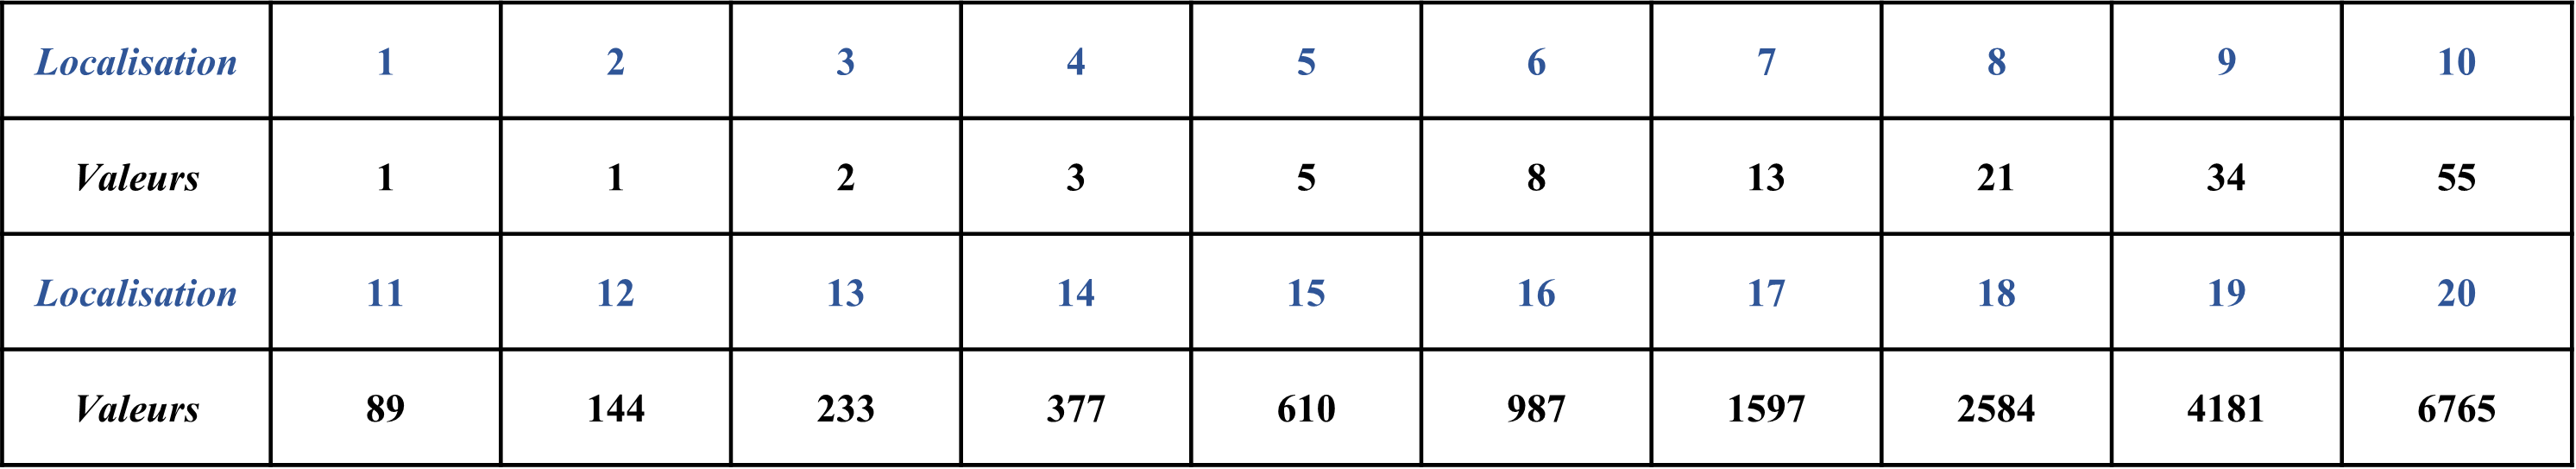
\includegraphics[scale =0.75]{Photos/Tableau Fibonacci.png}
        \label{tab:fibonacci}
    \end{table}
    \par
    D'après les résultats du tableau ci-dessus, nous pouvons voir que le résultat de l'opération respecte la règle selon laquelle le troisième terme est égal à la somme des deux premiers termes, nous considérons donc ce résultat comme acceptable.
    
    
    \subsection{Résultats d'un simulateur de population de lapins}
    \par
    Dans cette section, nous avons complété le simulateur pour les tests. Pour rendre reproductibles les résultats expérimentaux générés de manière aléatoire, nous avons utilisé un générateur de nombres pseudo-aléatoires MT\cite{matsumoto1998mersenne} de haute qualité. En outre, plusieurs expériences ont été réalisées pour réduire les erreurs dues aux expériences aléatoires. Cette section est donc divisée en deux parties, une pour l'expérience et une pour les résultats obtenus à partir d'expériences multiples.
    \subsubsection{Une expérience}
    \par
    Nous avons d'abord effectué un test unique sur le simulateur pour vérifier la faisabilité du modèle donné.\par
    \paragraph{Un couple de lapins adultes}\hspace{0.5cm}
    \newline
    \par La situation initiale de cette expérience ne comporte qu'un couple de lapins adultes et la simulation est effectuée sur 20 ans. Les résultats finaux que nous avons obtenus sont présentés dans le tableau \ref{fig3}.
    \begin{table}[!h]
	    \centering
	    \caption{Résultats d'une expérience de la croissance d'une population de lapins en débutant avec un couple unique de lapins adultes}
        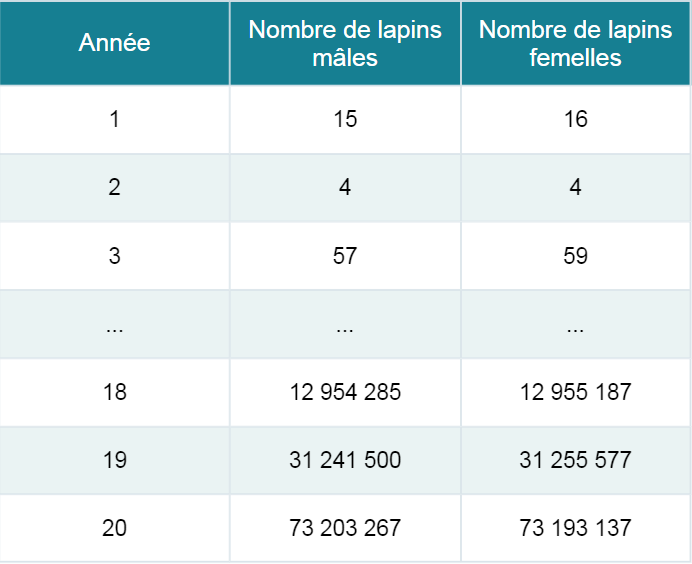
\includegraphics[scale = 0.7]{Photos/lapins1.png}
	    \label{fig3}
	\end{table}
    \par
    On observe que la population de lapin croît doucement au début puis très rapidement ensuite, jusqu'à doubler chaque année. On peut aussi remarquer que certaines années cette croissance est stoppée (par exemple entre l'année une et l'année deux). Ce phénomène peut s'expliquer par la très haute mortalité des bébés lapins qui constituent toujours une très grande partie de la population. Le hasard aurait pu décimer la population entière dès la deuxième année.\\
    \paragraph{Plusieur couples de lapins adultes}\hspace{0.5cm}
    \newline
    \par La situation initiale de cette expérience comporte dix couples de lapins adultes et la simulation est effectuée sur 20 ans. Les résultats finaux que nous avons obtenus sont présentés dans le tableau \ref{fig4}.
    \newpage
    \begin{table}[!h]
	    \centering
	    \caption{Résultats d'une expérience de la croissance d'une population de lapins en débutant avec dix couples de lapins adultes}
        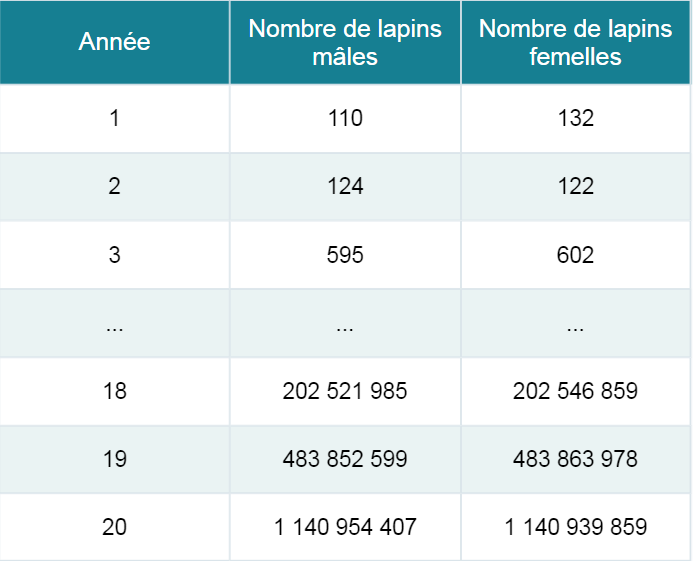
\includegraphics[scale = 0.7]{Photos/lapin10.png}
	    \label{fig4}
	\end{table}
    \par
    Ici, la croissance est toujours la même, le nombre de lapin semble souvent doubler d'une année sur l'autre. On a plus de dix fois plus de lapins à la fin de la simulation, ce qui semble être normal puisque nous avions dix fois plus de couples au départ.\\
    \par
    \paragraph{Un couple de petits lapins}\hspace{0.5cm}
    \newline
    \par Testons cette fois-ci avec seulement des bébé lapins au départ. La situation initiale de cette expérience ne comporte qu'un couple de petits lapins et la simulation est effectuée sur 20 ans. Les résultats finaux que nous avons obtenus sont présentés dans le tableau \ref{fig5}.
    \begin{table}[!h]
	    \centering
	    \caption{Résultats d'une expérience de la croissance d'une population de lapins en débutant avec un couple unique de petits lapins}
        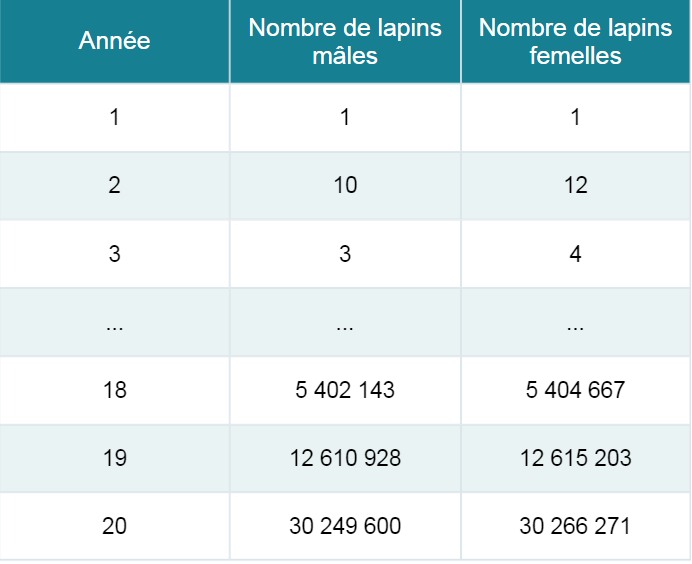
\includegraphics[scale = 0.7]{Photos/lapins1p.png}
	    \label{fig5}
	\end{table}
    \par
    On observe que la population de lapin croît bien plus doucement et que les petits lapins menacent de disparaître dès la première année à cause de leur forte mortalité. Cependant, s'il survivent, la simulation peut se poursuivre et beaucoup de lapins naissent aussi, ce qui permet d'arriver à une population tout de même importante à la fin de l'année 20.
    \paragraph{Plusieur couples de petits lapins}\hspace{0.5cm}
    \newline
    \par La situation initiale de cette expérience comporte dix couples de bébé lapins et la simulation est effectuée sur 20 ans. Les résultats finaux que nous avons obtenus sont présentés dans le tableau \ref{fig6}.
    \begin{table}[!h]
	    \centering
	    \caption{Résultats d'une expérience de la croissance d'une population de lapins en débutant avec dix couples de petits lapins}
        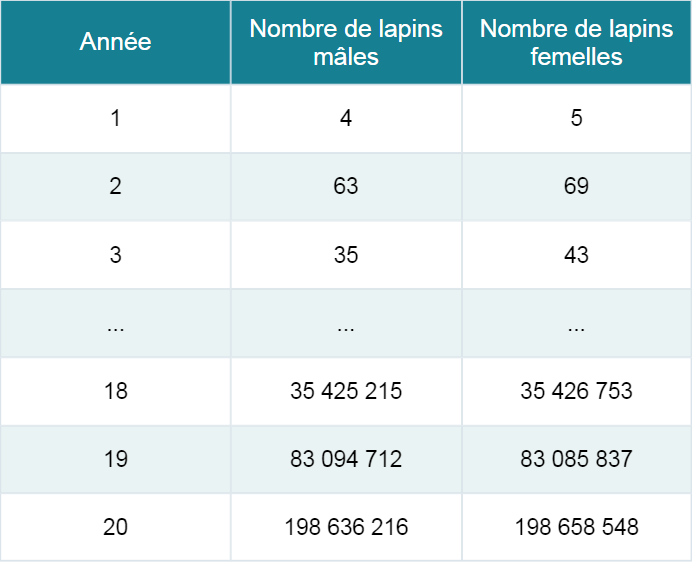
\includegraphics[scale = 0.8]{Photos/lapins10p.png}
	    \label{fig6}
	\end{table}
    \par
    Ici, on peut faire les même remarques car seulement la moitié des lapereaux survit à la première année. Cependant la croissance de la population reste très importante.
    \paragraph{Plusieur couples de petits lapins et de lapins adultes}\hspace{0.5cm}
    \newline
    \par La situation initiale de cette expérience-ci comporte deux couples de bébé lapins ainsi que deux couples de lapins adultes et la simulation est effectuée sur 20 ans. Les résultats finaux que nous avons obtenus sont présentés dans le tableau \ref{fig7}.
    \newpage
    \begin{table}[!h]
	    \centering
	    \caption{Résultats d'une expérience de la croissance d'une population de lapins en débutant avec deux couples de petits lapins et deux couples de lapins adultes}
        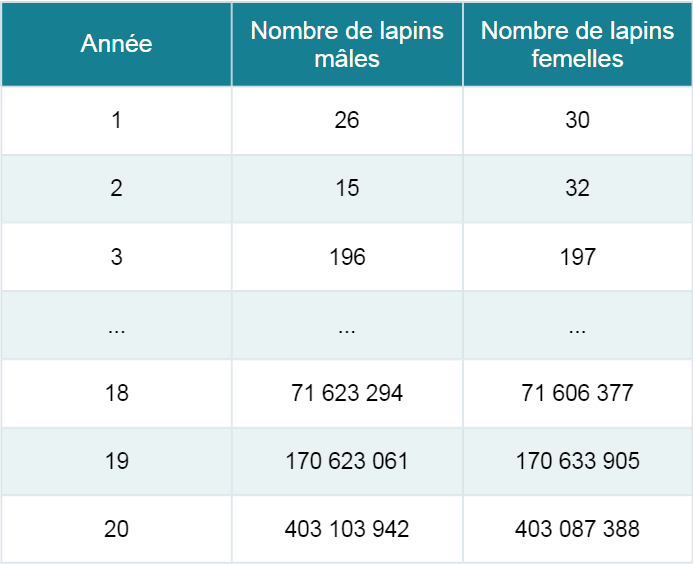
\includegraphics[scale = 0.7]{Photos/lapin2_2.png}
	    \label{fig7}
	\end{table}
    \par
    Avec cette expérience, on remarque que le risque de perdre tous les lapins dès la première année est très faible puisque la population explose dès le début grâce aux nombreux petits qu'engendrent les deux couples adultes.\\
    \par
    Ces expériences uniques sont cependant bien insuffisantes pour tirer de réelles conclusion, c'est pourquoi il faut en réaliser plusieurs indépendantes les unes des autres et faire une moyenne des résultats obtenus.
    \subsubsection{Plusieurs expériences}
    \par
    Ici, cent simulations sont effectuées et les valeurs résultantes sont moyennées afin de réduire l'erreur due aux essais aléatoires.

    \paragraph{Un couple de lapins adultes}\hspace{0.5cm}
    \newline
    \par Commençons par observer comment se débrouille en moyenne un couple unique de lapins adultes sur vingt ans. Les résultats finaux que nous avons obtenus sont présentés dans le tableau \ref{fig8}.
    \newpage
    \begin{table}[!h]
	    \centering
	    \caption{Résultats de la moyenne de cent expériences sur la croissance d'une population de lapins en débutant avec un couple unique de lapins adultes}
        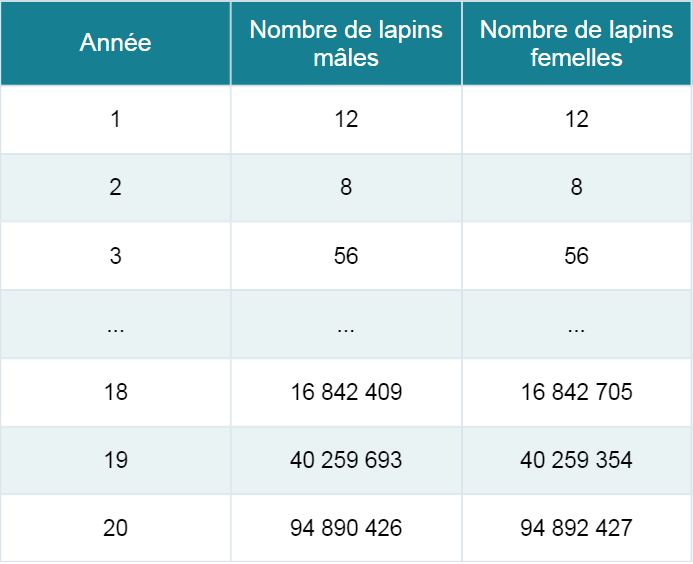
\includegraphics[scale = 0.68]{Photos/mean2Lap.png}
	    \label{fig8}
	\end{table}
    \par
    On observe ici qu'un seul couple de lapins adulte suffit à ce que la population grandisse rapidement, sans qu'il y ait un risque trop important de perdre tous les lapins d'un coup, notamment la première année. La forte mortalité des petits a un fort impact certaines fois, notamment sur l'année deux où on voit la population totale chuter, mais elle n'entrave pas complètement le développement de la population.
    \paragraph{Plusieur couples de lapins adultes}\hspace{0.5cm}
    \newline
    \par Cette expérience vise à observer le développement moyen de la population de lapins s'il y a maintenant dix couples de lapins adultes à l'origine. On observe les résultats suivants :
    \begin{figure}[!h]
	    \centering
	    
        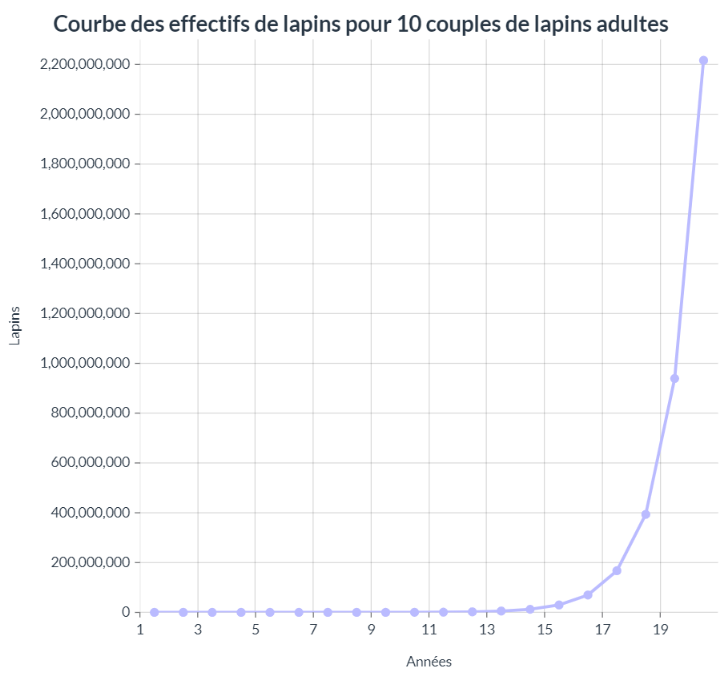
\includegraphics[scale = 0.6]{Photos/courbes10lap.png}
        \caption{Courbe réprésentant la moyenne de cent expériences sur la croissance d'une population de lapins en débutant avec dix couples de lapins adultes}
	    \label{fig9}
	\end{figure}
    \par
    On remarque une croissance exponentielle. Les lapins adultes ont moins de chance de mourir donc les dix couples font tout de suite exploser le nombre de lapins, ce dès la première année avec en moyenne une population de 251 lapins dès le début, soit le double de lapins. La deuxième année, beaucoup de petits sont morts donc la population baisse légèrement (244 lapins en moyenne), mais le nombre ne cesse d'augmenter à partir de là. La simulation est donc très intéressante avec plusieurs couples de lapins adultes.
    \par
    \paragraph{Un couple de petits lapins}\hspace{0.5cm}
    \newline
    \par Testons cette fois-ci avec seulement des bébés lapins au départ. Pour commencer, nous observerons comment la population se développe avec un seul couple au départ. Les résultats finaux que nous avons obtenus sont présentés dans le tableau \ref{fig10}.
    \begin{table}[!h]
	    \centering
	    \caption{Résultats de la moyenne de cent expériences sur la croissance d'une population de lapins en débutant avec un couple unique de petits lapins}
        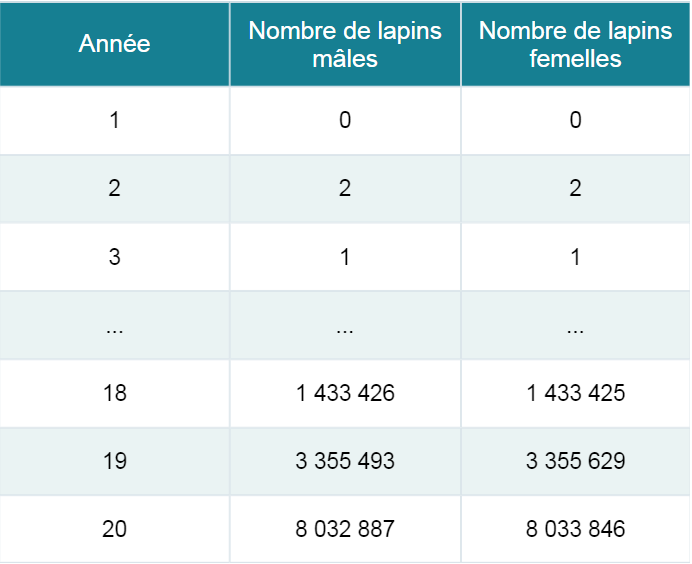
\includegraphics[scale = 0.8]{Photos/mean2LapP.png}
	    \label{fig10}
	\end{table}
    \par
    Ici, on voit qu'en moyenne le couple de lapin meurt dès la première année, ce qui stoppe totalement la croissance de la population. Il vaut donc mieux soit prendre des lapins adultes au départ, soit augmenter le nombre de couples de lapereaux pour voir la croissance de la population de lapins. Cependant, si le couple survit, au bout des vingt années de simulation, la population s'est tout de même beaucoup développée.
    \paragraph{Plusieur couples de petits lapins}\hspace{0.5cm}
    \newline
    \par La situation initiale de cette expérience comporte dix couples de bébé lapins et la simulation est effectuée sur 20 ans. On observe les résultats suivants :
    \newpage
    \begin{figure}[!h]
	    \centering
	    
        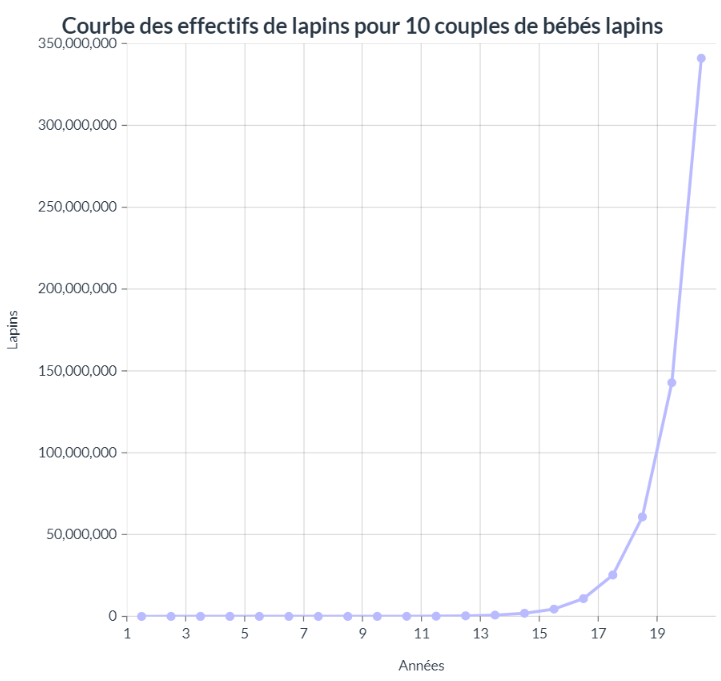
\includegraphics[scale = 0.8]{Photos/courbes10lapP.png}
        \caption{Courbe représentant la moyenne de cent expériences sur la croissance d'une population de lapins en débutant avec dix couples de petits lapins}
	    \label{fig11}
	\end{figure}
    \par
    On observe ainsi une croissance exponentielle de la population des lapins malgré la forte mortalité des petits. En effet, en moyenne, seuls trois couples survivent à la première année, mais c'est suffisant pour que la population puisse grandir, et ce très rapidement.
    \paragraph{Plusieur couples de petits lapins et de lapins adultes}\hspace{0.5cm}
    \newline
    \par On reprend ici deux couples de petits lapins et deux couples de lapins adultes pour observer comment se développe une population "mixte". Les résultats sont alors les suivants :
    \newpage
    \begin{figure}[!h]
	    \centering
	    \caption{Courbe représentant la moyenne de cent expériences sur la croissance d'une population de lapins en débutant avec deux couples de petits lapins et deux couples de lapins adultes}
        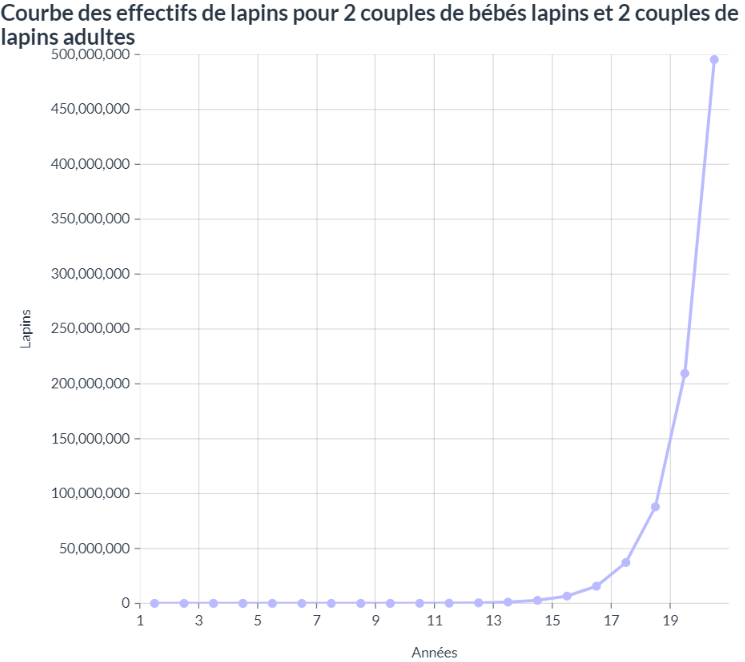
\includegraphics[scale = 0.8]{Photos/courbe2_2.png}
	    \label{fig12}
	\end{figure}
    \par
    Cette expérience montre qu'avec une population de départ "mixte", on minimise le risque de perdre toute la population dès le début (en moyenne, 51 lapins survivent à la première année) et on lui permet de croître très vite. Evidemment, le plus efficace pour avoir un grand nombre de lapins reste de prendre beaucoup de couples de lapins adultes.
    \newpage
    \section{Conclusion}
    \par
    Dans cette expérience, nous avons d'abord réalisé un générateur efficace de tableaux de Fibonacci. Ensuite, nous avons réalisé une simulation de population de lapins à l'aide du générateur de nombres pseudo-aléatoires MT. Dans ce simulateur, nous avons divisé en deux parties principales, le calcul du nombre de lapins nés et le calcul du nombre de lapins morts. Au final, plusieurs expériences ont été réalisées afin de minimiser les erreurs découlant des expériences aléatoires pour obtenir les résultats finaux.
    \par
    Le plus gros problème que nous avons rencontré au cours de l'expérience concernait le choix des unités de calcul. Nous avons passé beaucoup de temps à modéliser les différents états des lapins afin d'affiner la simulation. Cependant, en raison des problèmes décrits dans le document, nous avons finalement choisi d'utiliser l'année comme unité de calcul. Nous avons réalisé que, pour éviter cette situation, il fallait envisager l'ensemble du système dès le début de la mise en œuvre du logiciel.
    \par
    Notre mise en œuvre actuelle est un modèle de simulation de populations de lapins basé sur des nombres aléatoires. Après avoir obtenu ces données, nous pouvons les traiter encore davantage. Il existe une expérience similaire dans le domaine de l'intelligence artificielle qui simule les prix des maisons à Boston\cite{muralidharan2018analysis}. Ensuite, après avoir obtenu ces résultats générés de manière aléatoire sur la base de nombres aléatoires, nous pouvons utiliser une idée similaire et utiliser les données résultantes comme ensemble de données afin de compléter un réseau neuronal pour la simulation de la population de lapins.

    \newpage	    
    \bibliographystyle{ieeetr}
    \bibliography{ref}
    {\textcolor{blue}{*}} La configuration matérielle de l'ordinateur utilisée pour cette expérience était la suivante:
    \begin{itemize}
        \item Systèmes d'exploitation: Windows 11 Professionnel Version 22H2
        \item Unité de traitement centrale: Intel® Core™ i7-8750H
        \item Mémoire à accès aléatoire: Mémoire DDR4 monocanal de 16 Go
    \end{itemize}
    
    \label{lastPage}
    
\end{document}